\section{Il filtro}

Per l'elaborazione dei dati ricevuti dalle IMU è stato utilizzato il filtro complementare, che unisce un'implementazione relativamente semplice a dei risultati di performance comparabili a filtri più complessi, come il filtro di Kalman.\\

Esso si basa su un processo di \textit{sensor fusion} con il raggiungimento di una stima degli angoli di roll, pitch e yaw tramite due diversi approcci, per poi unire i due contributi a meno di una costante complementare $\alpha$ che esprime il grado di fiducia nel corrispettivo sensore.\\

In particolare, nel progetto in questione si è fatto anche riferimento all'articolo \cite{KOTTATH2017574}, che applica un filtro complementare leggermente diverso da quello canonico.

\begin{figure}[H]
    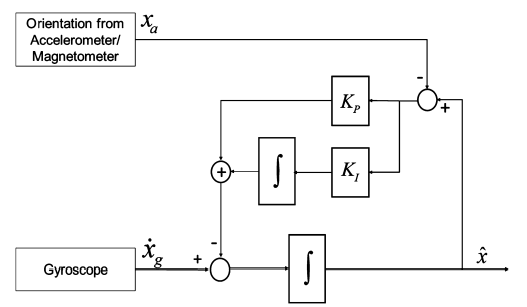
\includegraphics[scale=1]{immagini/filter.png}
    \centering
    \caption{Schema filtro complementare proposto}
\end{figure}

Nella prima parte, gli angoli vengono ottenuti dall'integrazione delle misure del giroscopio, paragrafo (\ref{Dati giroscopio}) equazioni (\ref{integr phi}) (\ref{integr theta}) e (\ref{integr psi}):\\

\begin{equation*}
    \begin{cases}
        \dot{\phi} = p + q \sin{\phi} \tan{\theta} + r \cos{\phi} \tan{\theta}\\
        \dot{\theta} = q \cos{\phi} - r \sin{\phi}\\
        \dot{\psi} = q \sin{\phi} \sec{\theta} + r \cos{\phi} \sec{\theta}
    \end{cases}
\end{equation*}\\

nella seconda parte, roll e pitch derivano da formule basate su considerazioni sulla gravità già discusse nel paragrafo (\ref{Dati accelerometro}) equazioni (\ref{eq phi roll acc}) e (\ref{eq theta pitch acc}); lo yaw, come già discusso nel paragrafo (\ref{Dati magnetometro}), necessita di un riferimento di \textit{heading} e quindi del magnetometro, paragrafo (\ref{Dati magnetometro}) equazione (\ref{eq psi yaw magn}):\\

\begin{equation*}
    \begin{cases}
        \phi_a = \tan^{-1} \begin{pmatrix} \frac{a_y}{a_z} \end{pmatrix}\\
        \theta_a = \tan^{-1} \begin{pmatrix} \frac{-a_x}{a_y \sin{\phi_a} \, + \, a_z \cos{\phi_a}} \end{pmatrix}\\
        \psi_m = \tan^{-1} \begin{pmatrix} \frac{m_x \sin{\phi_a} \, - \, m_y \cos{\phi_a}}{m_x \cos{\theta_a} \, + \, m_y \sin{\theta_a} \sin{\phi_a} \, + \, m_z \sin{\theta_a} \cos{\phi_a}} \end{pmatrix}
    \end{cases}
\end{equation*}\\


Infine quindi tali stime basate sui singoli sensori vengono unite: la formula classica (\cite{ahrs}, quaternioni) è
\begin{equation}
    \hat{q} = \alpha \, q_g + (1 - \alpha) \, q_{am}
\end{equation}

che in seguito è stata ripresa ed espansa (\cite{KOTTATH2017574}) come
\begin{equation}
    \hat{x}_{new} = \frac{1}{s} \begin{bmatrix} \dot{x}_g + (K_p + \frac{K_I}{s}) (x_{am} - \hat{x}) \end{bmatrix}
\end{equation}

e che rivista e semplificata ($K_I = 0$) diventa
\begin{equation}
    \hat{x}_{new} = \frac{1}{s} \begin{bmatrix} \alpha \, \dot{x}_g + (1 - \alpha) (x_{am} - \hat{x}) \end{bmatrix}
\end{equation}

dove 
\begin{equation}
    \dot{x}_g = \columnvector{\dot{\phi} \\ \dot{\theta} \\ \dot{\psi}} \quad , \quad x_{am} = \columnvector{\phi_a \\ \theta_a \\ \psi_m}
\end{equation}\\

$\hat{x}_{new}$ è la stima finale degli angoli di roll pitch e yaw, $\hat{x}$ è la stima allo step precedente, $\dot{x}_g$ sono le velocità angolari ricavate dai giroscopi dopo le correzioni di rotazione, e $x_{am}$ sono le misure ricavate da accelerometro e magnetometro.\\

La formula finale quindi risente di entrambi i metodi, dove la variabile proporzionale $K_p$ è stata riconvertita in $\alpha$.\\
È stato poi notato sperimentalmente che il valore migliore per $\alpha$ fosse più vicino a 1, e si assestasse su 0.9.\\

Le funzioni di filtraggio sono presenti nel codice python, in particolare il lavoro viene svolto dalla funzione \mcode{Complementary2eul()}.

\begin{figure}[H]
    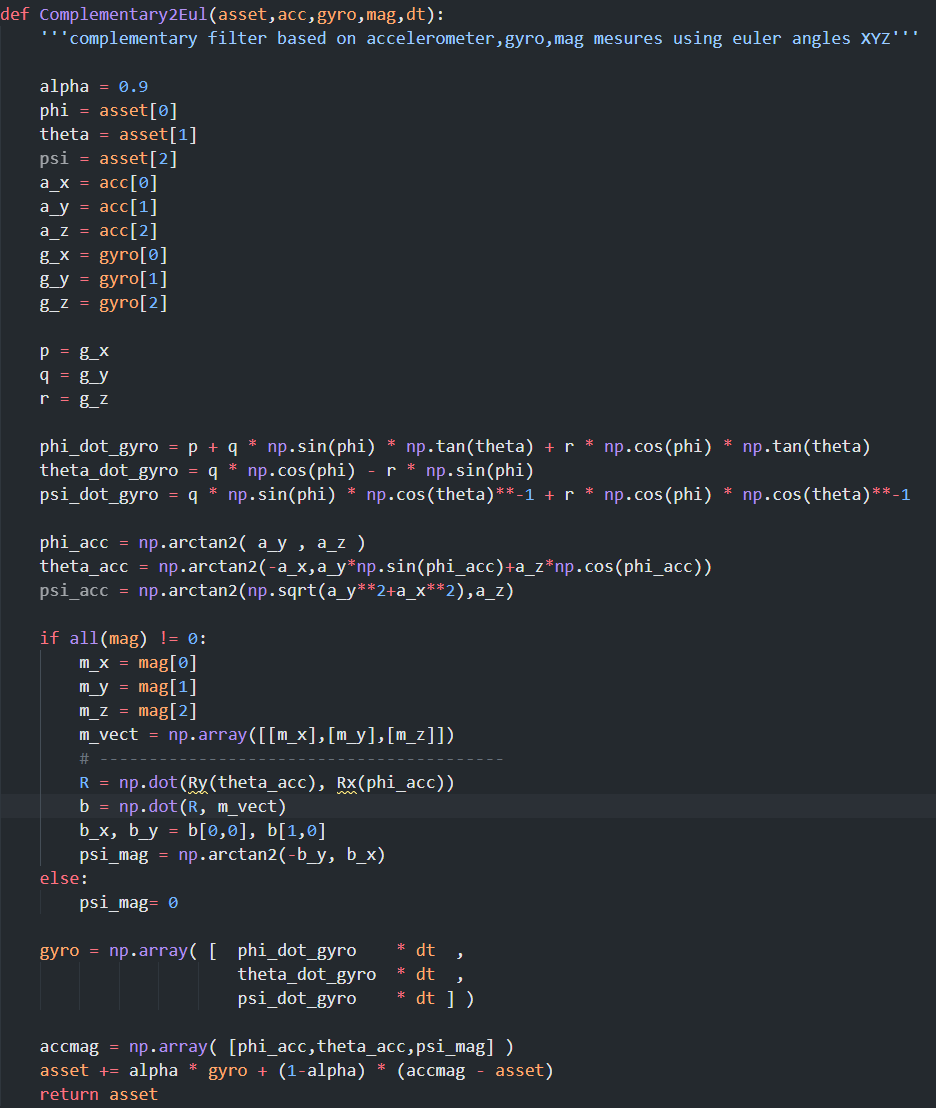
\includegraphics[scale=0.6]{immagini/filtercode.png}
    \centering
    \caption{Codice del filtro complementare.}
\end{figure}

\clearpage